\documentclass[letterpaper, twoside, 12pt,memoire]{thETS}
\usepackage{amsmath}
\usepackage{amsfonts}
\usepackage{amssymb}
\usepackage[utf8]{inputenc}
\usepackage{graphicx}
\usepackage{color}
\usepackage[T1]{fontenc}
\usepackage{subfigure}
\usepackage{setspace}
\usepackage{todonotes}
\usepackage{varwidth}
\usepackage{float}
\usepackage[section]{placeins}
\usepackage[round]{natbibETS}
%\usepackage{url}
\usepackage{MyAlgorithmic}
\usepackage[chapter]{MyAlgorithm}
\usepackage[mathcal]{euscript}
 

%DIF 22c22-23
%DIF < \hyphenpenalty=5000 \tolerance=1000
%DIF -------
\hyphenpenalty=5000 %DIF > 
\tolerance=1000 %DIF > 
%DIF -------

\newcommand{\LT}[1]{%
	{
	\todo[inline,color={red!33!green!33!blue!33}]{%
	\textbf{[LT]:}~#1}
	}}
	
\newcommand{\SC}[1]{%
	{
	\todo[inline,color={red!100!green!33!}]{%
	\textbf{[SC]:}~#1}
	}}

\newcommand{\fig}[1]{figure~\ref{#1}}
\newcommand{\ltF}[1]{\mathbf{F}_{#1}}
\newcommand{\ltE}[1]{\mathbf{E}_{#1}}
\newcommand{\ltP}[1]{\mathbf{P}_{#1}}
\newcommand{\ltD}[1]{\mathbf{D}_{#1}}
\newcommand{\ltS}[1]{I_{#1}}

%DIF 43a44
\newcommand{\ltDiffBad}{\left| \ltE{x,y} - \ltP{x,y} \right|} %DIF > 
%DIF -------
\newcommand{\ltDiffGood}{\left| \ltF{x,y} - \ltP{x,y} \right|}

\newcommand{\ltCodec}{logiciel de référence H.264/AVC JM}

\newcommand{\ltSAD}[1]{\textrm{SAD}(#1)}
\newcommand{\ltMIN}[1]{\arg \min_{#1}}
\newcommand{\lttBLK}[2]{\textrm{MCB}_{#1}(#2)}
\newcommand{\ltCB}[2]{\mathbf{b}_{#1}(#2)}
\newcommand{\ltSTBLK}[1]{\textrm{SMCB}(#1)}
\newcommand{\ltBor}[1]{\mathcal{#1}}

\newcommand{\ltSDMCB}[1]{\textrm{SDMCB}(#1,\ltP{},m,n)}
\newcommand{\ltErr}[1]{\mathbf{\hat{F}}_{#1}}
\newcommand{\ltConc}[1]{\mathbf{F^{\prime}}_{#1}}
\newcommand{\ltOpt}[1]{\mathbf{F^{*}}_{#1}}

\newcommand{\sect}[1]{section~\ref{#1}}
%DIF PREAMBLE EXTENSION ADDED BY LATEXDIFF
%DIF UNDERLINE PREAMBLE %DIF PREAMBLE
\RequirePackage[normalem]{ulem} %DIF PREAMBLE
\RequirePackage{color}\definecolor{RED}{rgb}{1,0,0}\definecolor{BLUE}{rgb}{0,0,1} %DIF PREAMBLE
\providecommand{\DIFadd}[1]{{\protect\color{blue}\uwave{#1}}} %DIF PREAMBLE
\providecommand{\DIFdel}[1]{{\protect\color{red}\sout{#1}}}                      %DIF PREAMBLE
%DIF SAFE PREAMBLE %DIF PREAMBLE
\providecommand{\DIFaddbegin}{} %DIF PREAMBLE
\providecommand{\DIFaddend}{} %DIF PREAMBLE
\providecommand{\DIFdelbegin}{} %DIF PREAMBLE
\providecommand{\DIFdelend}{} %DIF PREAMBLE
%DIF FLOATSAFE PREAMBLE %DIF PREAMBLE
\providecommand{\DIFaddFL}[1]{\DIFadd{#1}} %DIF PREAMBLE
\providecommand{\DIFdelFL}[1]{\DIFdel{#1}} %DIF PREAMBLE
\providecommand{\DIFaddbeginFL}{} %DIF PREAMBLE
\providecommand{\DIFaddendFL}{} %DIF PREAMBLE
\providecommand{\DIFdelbeginFL}{} %DIF PREAMBLE
\providecommand{\DIFdelendFL}{} %DIF PREAMBLE
%DIF END PREAMBLE EXTENSION ADDED BY LATEXDIFF

\begin{document}
\begin{chapter}{Une nouvelle approche d'identification et de dissimulation de la
détérioration visuelle}

Les chapitres antérieurs constituent les éléments d'un panorama technologique
permettant l'assimilation des notions présentées dans ce chapitre. Ces éléments
recouvrent un large territoire technologique s'étendant de l'encodage vidéo, au
transport de celui-ci ainsi que l'impact, la détection et la dissimulation
de la détérioration de séquences vidéos codées en respectant la norme H.264.

Rappelons d'abord, à la \sect{sect-limitations}, les limitations des
approches actuelles de détection d'erreurs. Nous présentons ensuite, à la
\sect{sect-MCB}, une amélioration fondamentale aux approches actuelles de
détection de la dégradation visuelle à l'intérieur de trames corrompues.
Cette approche de détection améliorée sert de base pour un nouveau type d'approche de dissimulation,
les approches sélectives. À la \sect{sect-Selectives}, deux variantes de
celles-ci sont décrites.

\begin{section}{Les limitations des approches actuelles de détection de la
détérioration visuelle}
\DIFaddbegin \label{sect-limitations}
\DIFaddend Les approches de détection de la détérioration visuelle étudiées ici sont
celles présentées lors de notre revue de la littérature. Avant de définir les
limitations de ces approches, commençons par uniformiser la nomenclature
utilisée pour décrire celles-ci. Définissions deux matrices : $\ltF{}$, celle
contenant les pixels d'une trame d'une séquence vidéo et $\ltE{}$ la matrice
de pixels issue du décodage réussi des paquets de $\ltF{}$, corrompus lors du transport. Pour une matrice $\ltF{}$, $\ltF{x,y}$ représente la valeur du pixel de la matrice à la position $(x,y)$.
\DIFaddbegin \SC{On ne peut pas parler de paquets de $\ltF{}$ car $\ltF{}$ est une matrice. Selon moi il faudrait citer une figure de diagramme de système avec les matrices définies ici ainsi que les autres que tu définiras. Genre $\ltF{O}$ est ton image originale, elle est codée en $\ltF{}$ et brisée en paquets $p_i(\ltF{})$ qui sont corrompus et appelés $\hat{p}_i(\ltF{})$ ou quelque chose du genre. Ici il faudrait aussi séparer ce qui est une notation (par exemple $\ltF{}$  est une matrice et $\ltF{x,y}$ est la valeur à la position $(x,y)$ est une notation générale) de la liste des signaux à définir: $\mathbf{F,E,P,... }$. Selon moi, c'est pour cela qu'une figure du système avec les signaux  $\mathbf{F,E,P,... }$ est requise  ou au moins les définir. Pour la notation matrice pas besoin de définir pour F et E juste un des deux (ou une matrice générique F). Tu pourrais définir $\ltF{O}(t)$ la trame originale au temps $t$ (pas compressée), $\mathbf{F}(t)$ la trame encodée et décodée sans erreur au temps $t$,  $\mathbf{\hat{F}}(t)$ la trame encodée, transmise, puis décodée au temps $t$ (donc possiblement corrompue). Et tu dirais que pour alléger la notation, lorsque le contexte sera clair, on notera: $\ltF{}$ pour $\mathbf{{F}}(t)$ la trame courante,$\ltE{}$ pour $\mathbf{\hat{F}}(t)$ la trame courante erronée, $\ltP{}$ pour $\mathbf{{F}}(t-1)$ la trame précédente (car on fait l'hypothèse qu'elle est sans erreur), etc. }
\DIFaddend 

Les auteurs, \citet{Superiori2007} ainsi que \citet{Ikuno2007}, présentent une
approche de détection où l'on mesure l'énergie des blocs ainsi que leurs effets
de blocs à l'intérieur d'un différentiel $\ltD{}$. Ce différentiel, issue de la
différence absolue entre la trame erronée $\ltE{}$ et la trame qui la précède
$\ltP{}$, est défini par la formule suivante~:
\begin{equation}
\DIFdelbegin %DIFDELCMD < \ltD{} %%%
\DIFdelend \DIFaddbegin \ltD{x,y} \DIFaddend = \DIFdelbegin %DIFDELCMD < \left| \ltE{} %%%
\DIFdel{- }%DIFDELCMD < \ltP{} \right|%%%
\DIFdelend \DIFaddbegin \ltDiffBad\:\DIFaddend ,
\end{equation}

Les données obtenues par ces mesures sont comparées à des seuils et un système
de votes détermine s'il y a erreur. La méthode se base sur l'hypothèse que les pixels ne varient pas beaucoup d'une image à l'autre et que les grandes variations sont probablement dues à des erreurs de transmission. Nous présentons, à titre d'exemple de cette
approche, la \fig{fig-FrameDiff} tirée de \citet[p.~25]{Ikuno2007}. Pour éviter
le recours aux seuils, les auteurs \citet{Farrugia2008} collectent une série de
mesures provenant de $\ltD{}$ et utilisent une machine à vecteurs de support
\citep{SVM1995} pour identifier les blocs erronés.

\begin{figure}
\fbox{\begin{varwidth}{\textwidth}\centering
\subfigure[$\ltD{}$]{
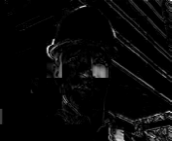
\includegraphics[width=0.30\linewidth]{images/FrameDifference.png}
\label{fig-Diff}
}
\subfigure[Analyse du différentiel]{
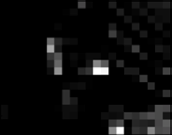
\includegraphics[width=0.30\linewidth]{images/FrameDifferenceAnalysis.png}
\label{fig-DiffAnalysis}
}
\subfigure[Erreurs détectées]{
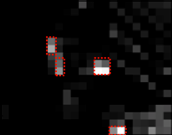
\includegraphics[width=0.30\linewidth]{images/FrameDifferenceDetection.png}
\label{fig-DiffDetection}
}
\end{varwidth}}
\caption{Exemple de l'analyse et de la détection d'erreurs.
\\Tirée de \citet[p.~25]{Ikuno2007}}
\label{fig-FrameDiff}
\end{figure}
\DIFaddbegin \SC{Ce serait bien de voir l'image E et P}
\DIFaddend 

Le problème commun que nous identifions, comme limitation majeure, avec ces
approches est l'usage du différentiel $\ltD{}$. Quoiqu'il puisse sembler
alléchant, ce dernier, illustré à la \fig{fig-Diff}, ne contient pas uniquement
l'erreur due aux erreurs de transmission, mais aussi la variation des valeurs de pixels propre à la séquence.
C'est-à-dire que le différentiel résultant des transformations entre les images non erronées, 
entre $\ltF{}$ et $\ltP{}$, tel le mouvement des objets, est aussi contenu dans $\ltD{}$. En effet, utilisant l'inégalité du triangle ( $\left|a-b\right| \le\left|a-c\right| + \left|c-b\right| $), on peut réécrire l'équation précédente comme:

\begin{equation}
\ltD{}= \left|\ltE{}-\ltP{}\right| \le   \underbrace{ \left|\ltE{}-\ltF{}\right|}_{\ltD{e}} +   \underbrace{ \left|\ltF{}-\ltP{}\right|}_{\ltD{v}} 
\end{equation}

avec $\ltD{e}$ l'erreur produite par les détériorations visuelles due aux erreur de transmission et $\ltD{v}$ l'erreur produite par les variations entre les trames.  On peut remarquer que sans $\ltF{}$, il est impossible de distinguer, à l'intérieur
de $\ltD{}$, les contributions individuelles de $\ltD{e}$ et de $\ltD{v}$. Les auteurs mentionnés précédemment (\citet{Superiori2007},
\citet{Ikuno2007} ainsi que \citet{Farrugia2008}) misent sur les
caractéristiques spatiales de la dégradation visuelle pour tenter d'effectuer
cette distinction. Cependant, il est probable que la variation entre les trames
$\ltD{v}$ manifeste ce genre de caractéristiques. Comme nous le démontrons
aux figures~\ref{fig-CoastDiffGood} et \ref{fig-CoastDiffBad}.

\begin{figure}
\fbox{\begin{varwidth}{\textwidth}\centering
\subfigure[$\ltE{}$]{
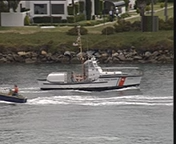
\includegraphics[width=0.47\linewidth]{images/coastguardBad.png}
\label{fig-CoastBad}
}
\subfigure[$\ltD{v}$]{
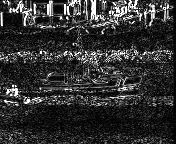
\includegraphics[width=0.47\linewidth]{images/coastguardDiffGood.png}
\label{fig-CoastDiffGood}
}
\subfigure[$\ltD{}$]{
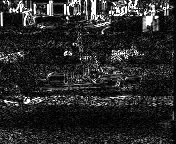
\includegraphics[width=0.47\linewidth]{images/coastguardDiffBad.png}
\label{fig-CoastDiffBad}
}
\subfigure[$\ltD{e}$]{
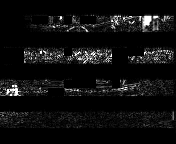
\includegraphics[width=0.47\linewidth]{images/coastguardDiffDiff.png}
\label{fig-CoastDiffDiff}
}
\end{varwidth}}
\caption{Contre-exemple de l'usage de $\ltD{}$ pour effectuer la détection
d'erreurs.}
\label{fig-Coastguard}
\end{figure}
\DIFaddbegin \SC{peux-tu remplacer remplacer la figure d) pour avoir $ \ltD{e}= |\ltE{}-\ltF{}|$ plutot que $\ltD{} - \ltD{v}\le  \ltD{e}$ }
\DIFaddend 

Par notre contre-exemple, la \fig{fig-Coastguard}, nous démontrons
l'inefficacité de la détection d'erreurs par $\ltD{}$. La séquence
\textit{coastguard} est caractérisée par un déplacement horizontal de la caméra.
Ce déplacement crée une très grande variation entre deux trames consécutives,
comme illustré à la \fig{fig-CoastDiffGood}. L'erreur à détecter est identifiée
à la \fig{fig-CoastDiffDiff}. Il n'est pas évident d'extraire cette information
de $\ltD{}$ (\fig{fig-CoastDiffBad}) sans connaitre $\ltF{}$.

Bref, ce manque de précision, engendré par la variation \textit{intertrame}
présente dans le différentiel, force les auteurs à employer des systèmes
complexes de votes ou de machines à vecteur de support. À l'opposé, le résultat
de notre effort de recherche est une approche de détection simple qui oeuvre dans
un contexte différent de $\ltD{}$, où la variation entre les trames est
minimisée par la compensation de mouvement.
\FloatBarrier
\end{section}

\begin{section}{Les effets de blocs compensés par le mouvement}
\label{sect-MCB}
Nous venons de présenter la variation entre les trames comme un obstacle majeur
à la détection d'erreurs. En s'intéressant aux origines de cette variation, on
constate qu'elle peut provenir: d'une translation, d'une déformation, d'un
changement intensité lumineux ainsi que de l'insertion ou du retrait de contenu.

\LT{Faire le lien avec le section sur les erreurs dans le vidéo.}

En pratique, l'erreur de transmission agit comme un changement entre les trames équivalant soit
à une déformation ou une insertion de contenu. Ce qui fait en sorte que ces
types de changements sont les plus difficiles à distinguer de l'erreur.

Dans le domaine de l'encodage vidéo numérique, la variation entre les trames est
un concept qui a suscité une grande quantité d'efforts de recherche. Comme
présentées dans notre section sur H.264, les approches de recherche et de
compensation de mouvement sont raffinées, depuis maintenant plusieurs années,
pour modéliser cette variation afin d'augmenter le taux de compression issue de
leur encodage.

\LT{Faire le lien avec la formule de recherche de mouvement du chapitre sur
H.264}

Dans notre contexte, ces algorithmes peuvent servir à prendre en compte les
changements entre les trames au lieu de les ignorer, comme c'est le cas avec les
approches qui reposent sur $\ltD{}$. La \fig{fig-BlockEnery} illustre bien que
l'erreur, présentée à la \fig{fig-CoastDiffDiff}, est mieux identifiée par l'erreur de prédiction associée à la l'estimation du mouvement, nommée résiduel~\ref{fig-BlockResidual} (où seul le
bloc erroné a une valeur supérieure à 3500) que par $\ltD{}$~\ref{fig-BlockDiff}
(où plusieurs blocs offrent des pointages excédant largement à celui de
l'erreur).
\DIFdelbegin %DIFDELCMD < 

%DIFDELCMD < %%%
\DIFdelend \DIFaddbegin \SC{Le lecteur ne peux pas comprendre ni ce paragraphe ni cette figure. le caption est à revoir aussi. la figure montre rouge et rouge. le lecteur ne sera pas convaincu. }
\DIFaddend \begin{figure}
\fbox{\begin{varwidth}{\textwidth}\centering
\subfigure[Somme des blocs $16\times16$ de $\ltD{}$]{
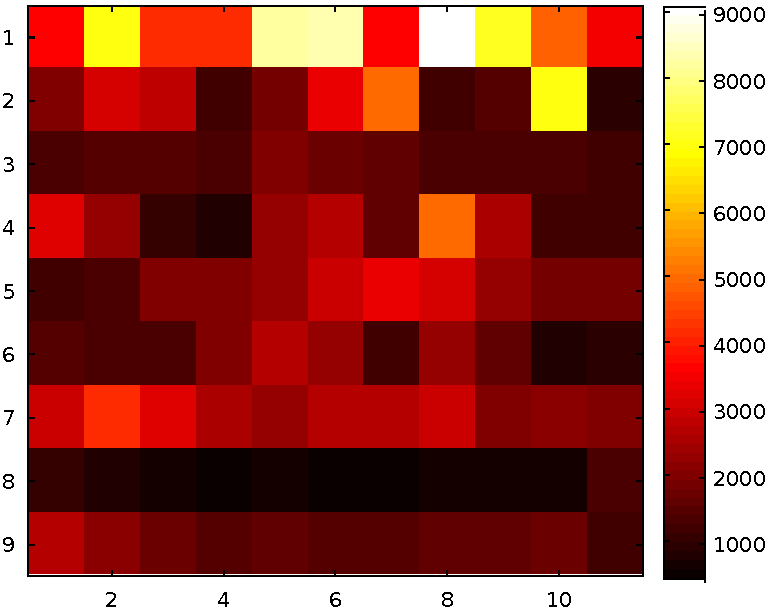
\includegraphics[width=0.47\linewidth]{images/blockDiff.pdf}
\label{fig-BlockDiff}
}
\subfigure[Somme des blocs $16\times16$ du résiduel]{
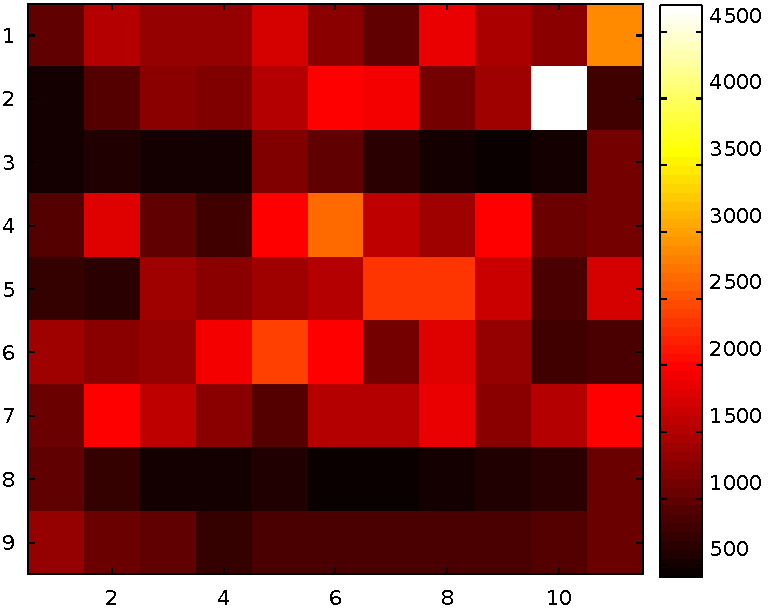
\includegraphics[width=0.47\linewidth]{images/blockResidual.pdf}
\label{fig-BlockResidual}
}
\end{varwidth}}
\caption{Résultats de la sommation des pixels contenus dans les macroblocs de
$\ltD{}$~\subref{fig-BlockDiff} et du résiduel\subref{fig-BlockResidual} sur la
\fig{fig-CoastBad}.}
\label{fig-BlockEnery}
\end{figure}

Quoiqu'elle améliore la détection d'erreurs, la compensation de mouvement n'est
pas en mesure d'identifier les vecteurs de mouvement corrompus\DIFaddbegin \SC{Je suis perdu, la compensation du mouvement sert au codage. pourquoi on parle de compensation de mouvement en lien avec les VM corrompus? est-ce que le lecteur a le background dans les autres chapitres?}\DIFaddend . Comme décrit au
chapitre \ref{chap-erreur}, ce type d'erreur insère du contenu fautif dans
l'image erronée, provenant du mauvais endroit dans la trame de référence. Pour
ce genre d'erreur, la recherche de mouvement retrouve le mauvais contenu et
n'est pas en mesure d'identifier l'erreur.\DIFaddbegin \SC{il trouve du contenu mais c'est le mauvais contenu qu'il utilise pour sa prédiction}
\DIFaddend 

\LT{Ajouter référence sur le chapitre des erreurs.}

Cette limitation de la recherche de mouvement nous apporte à incorporer un
élément important pour la détection d'erreurs. La notion de nuisance. Ce que
nous cherchons à détecter n'est pas l'erreur absolue, mais bien l'erreur qui
engendre une dégradation visuelle perceptible par le système visuel humain. Dans
le chapitre sur l'effet des erreurs sur les séquences vidéo, nous avons conclu
que pour être dérangeantes, les erreurs doivent exhiber un ou plusieurs effets
de blocs.

\begin{figure}
\fbox{
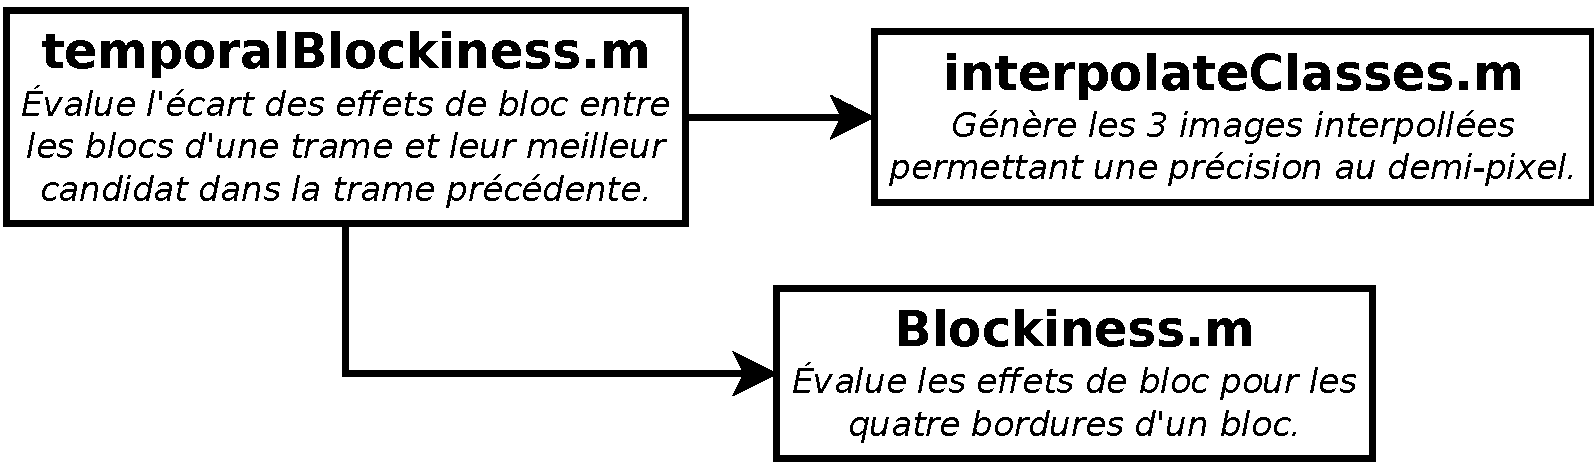
\includegraphics[width=0.97\linewidth]{images/MCB.pdf}
}
\caption{Visualisation des composantes liées au calcul du MCB.}
\label{fig-MCB}
\end{figure}
\DIFaddbegin \SC{changer évaluers par evaluer. doit-on dire trame à encoder ou trame à décoder?}
\DIFaddend 

Les effets de blocs compensés par le mouvement (MCB), que nous proposons dans cette recherche, sont la combinaison de
ces deux faits. Comme décris à la \fig{fig-MCB}, le MCB recherche les
discontinuités spatiales en bordure de blocs entre la trame à encoder et la
trame de référence. Ne connaissant pas la trame de référence, nous utilisons la
trame précédente.

Avant de procéder à l'explication pratique du fonctionnement du MCB (à la
sous-section \ref{subsect-ExplicationMCB}), nous présentons en détail, à la
section \ref{subsect-theorique}, sa définition mathématique afin de bien
comprendre comment le MCB est mesuré.

\FloatBarrier
\begin{subsection}{Définition théorique du MCB}
\label{subsect-theorique}
Pour cette démonstration et à des fins de simplicité, nous avons recours à des
blocs carrés\footnoteETS{Il est aussi possible d'utiliser des blocs
rectangulaires.} de taille $B$. Nous définissons un bloc comme un ensemble de pixels de taille
$B\times B$. La hauteur et la largeur d'une trame sont définies, respectivement,
par $H$ et $W$. Les intervalles $\ltS{m}=[0,\frac{W}{B}-1]$ et
$\ltS{n}=[0,\frac{H}{B}-1]$ représentent les indices de blocs à l'intérieur
d'une trame. Nous désignons $p$, comme la demi-hauteur de la fenêtre de
recherche de mouvement.

Nous employons $(u,v)$, comme le vecteur optimal issu de la recherche de
mouvement. Cette opération s'exprime par la formule suivante~: 
\begin{equation}
\label{eq-Vectors}
(\mathbf{U}_{m,n}, \mathbf{V}_{m,n}) = \ltMIN{(u,v) \in K} ~ \ltSAD{mB, nB, u,
v, \ltE{}, \ltP{}} \:,
\end{equation}
où $K = [-p,p] \times [-p, p]$,  $m \in \ltS{m}$, $n \in
\ltS{n}$ et
\begin{equation}
\label{eq-SAD}
\ltSAD{x,y,u,v, \ltE{}, \ltP{}} = \sum_{q=0}^{B-1}\sum_{r=0}^{B-1} \left|
\ltE{x+q,y+r} - \ltP{x+q+u,y+r+v} \right|\:.
\end{equation}

Les composantes des vecteurs de mouvements optimaux $(u,v)$ sont insérées à l'intérieur
des matrices $\mathbf{U}_{}$ et $\mathbf{V}_{}$, à la position correspondante à
l'indice du bloc. Cette opération est effectuée sur l'ensemble des blocs qui
composent la trame $\ltE{}$. Comme il a déjà été mentionné, nous effectuons la
recherche de vecteurs de mouvement afin de tenir compte des variations issues de
$\ltD{v}$ afin de les séparer de la mesure de détérioration visuelle. Ainsi, au lieu de faire une différence entre les blocs situés à la même position spatiale, notre métrique effectuera la différence sur les blocs correspondants d'une trame à l'autre en considérant le mouvement de ceux-ci. De cette manière, nous réduisons l'effet du mouvement des objets entre les trames  sur la mesure de différence.\DIFaddbegin \SC{pixel entier, quart, demi pixel?}
\DIFaddend 

Pour établir l'appariement des blocs entre la trame erronée et la trame de
référence, nous avons recours à la somme de la différence absolue~(SAD) entre
deux blocs~(eq.\ref{eq-SAD}). Quoiqu'il n'en résulte pas une identification
exacte du mouvement, cette approche est peu complexe et permet l'identification
du bloc candidat avec la plus faible variation par rapport au bloc désiré. Ainsi, lorsque, pour un bloc donné le SAD minimum est élevé, on peut souvent conclure qu'une erreur s'est produite.

Toutefois, l'usage du SAD minimum, tel que calculé en (\ref{eq-Vectors}), comme approche de détection d'erreurs n'est pas efficace lorsque le contenu erroné est présent dans la trame précédente $\ltP{}$ (c.-à-d. lorsqu'un bloc possède un bloc similaire dans la trame précédente). Cette situation se présente souvent lorsque les vecteurs de mouvement sont corrompus. Dans cette
situation, ces vecteurs pointent sur le mauvais contenu même si le SAD est faible, ce qui peut souvent
entrainer des effets de blocs importants.

C'est pour cette raison que, comme illustré à la \fig{fig-MCB}, nous mesurons plutôt
les effets de blocs en bordure du bloc à évaluer, par rapport aux effets de
blocs du candidat, indiqué par le vecteur $(u,v)$, résultant de la recherche de
mouvement (eq.\ref{eq-Vectors}). Nous nommons cette opération : la mesure
d'effets de bloc compensés par le mouvement. On y réfère aussi par son acronyme
anglais MCB, et elle est définie par la formule~:
\begin{equation}
\label{eq-blk}
\lttBLK{d}{\ltE{},\ltP{}, m,n} = \\ \sum_{l = 0}^{B-1} | \ltCB{d,l}{\ltE{},m B,n
B} - \ltCB{d, l}{\ltP{},m B+\mathbf{U}_{m, n}, n B +\mathbf{V}_{m, n}} |\:,
\end{equation}
où \mbox{$m \in \ltS{m}$}, \mbox{$n \in \ltS{n}$}. De plus, $\mathbf{U}$ et
$\mathbf{V}$ proviennent de l'équation~\eqref{eq-Vectors}. Le MCB est appliqué à
toutes les bordures d'un bloc ($d \in \mathcal{B}$). Nous référons aux bordures
d'un bloc par l'ensemble suivant~: $\mathcal{B}=\{\ltBor{N}, \ltBor{E},
\ltBor{S}, \ltBor{W}\}$ et nous mesurons les vecteurs d'effets de bloc
$\mathbf{b}_{d, l}$ pour chacune d'elles, à l'aide de:
\begin{align}
\ltCB{\ltBor{N}, l}{\ltF{}, x,y} &= \ltF{x+l,y} - \ltF{x+l,y-1}\:, \\
\ltCB{\ltBor{E}, l}{\ltF{}, x,y} &= \ltF{x+B,y+l} - \ltF{x+B-1,y+l}\:, \\
\ltCB{\ltBor{S}, l}{\ltF{}, x,y} &= \ltF{x+l,y+B} - \ltF{x+l,y+B-1}\:, \\
\ltCB{\ltBor{W}, l}{\ltF{}, x,y} &= \ltF{x,y+l} - \ltF{x-1,y+l}\:,
\end{align}
où $l \in [0, B-1]$, et $(x,y)$ sont les
coordonnées en pixels des blocs.

Pour évaluer l'effet global des effets de blocs en bordure d'un bloc, nous utilisons la somme des effets de blocs compensés par
le mouvement de ce dernier ($\textrm{SMCB}$). Cette mesure est obtenue, pour un
bloc aux coordonnées de bloc $(m,n)$, à l'aide de la formule suivante~:
\begin{equation}
\label{eq-SumTB}
\ltSTBLK{\ltF{},\ltP{}, m,n} =
\sum_{d\:\in\:\mathcal{B}}\lttBLK{d}{\ltF{},\ltP{},m,n}\:.
\end{equation}

Dans cette formule, on effectue la sommation des valeurs MCB pour chacune des
bordures $d \in \mathcal{B}$ du bloc évalué. Ce qui est intéressant avec cette nouvelle approche c'est que nous mesurons le niveau de discontinuité présent à la bordure du bloc calculé par la soustraction du bloc considéré et le bloc qui lui correspond le mieux dans l'image précédente. S'il n'y aucun bloc correspondant bien ou si le bloc correspond bien mais provient de l'application d'un mauvais vecteur de mouvement et qu'il est ainsi hors de son contexte initial, la mesure sera élevée. Sinon, si un objet s'est seulement déplacé et ainsi le contexte visuel est le même autour du bloc considéré et son bloc correspondant, et ce même s'il y a beaucoup de détails ou des bordures marquées autour de ces blocs, alors la mesure sera faible par l'effet soustractif de la mesure.\DIFaddbegin \SC{une figure pour illustrée ces cas?}
\DIFaddend 

La détection d'effets de bloc par la mesure de pixels en bordure de blocs peut toutefois
introduire de fausses détections pour les bordures de blocs avoisinant un bloc
erroné. Comme illustré à la \fig{fig-GridSMCB}, dans une telle situation, la
valeur du SMCB des blocs voisins à la détérioration visuelle est
considérablement augmentée par la bordure limitrophe à l'erreur.

\begin{figure}
\fbox{\begin{varwidth}{\textwidth}\centering
\subfigure[Valeurs MCB et SMCB]{
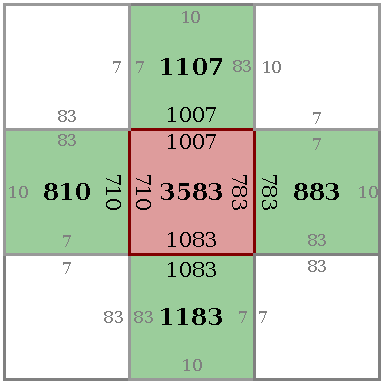
\includegraphics[width=0.40\linewidth]{images/Grid3x3_SMCB.pdf}
\label{fig-GridSMCB}
}
\subfigure[Valeurs distribuées MCB et SMCB]{
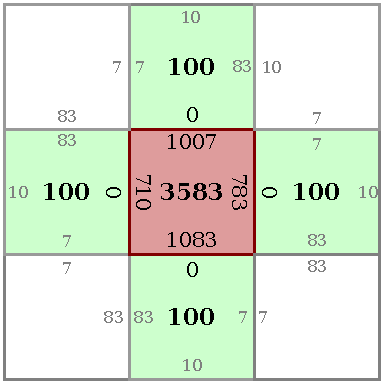
\includegraphics[width=0.40\linewidth]{images/Grid3x3_SDMCB.pdf}
\label{fig-GridSDMCB}
}
\subfigure{
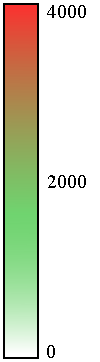
\includegraphics[width=0.11\linewidth]{images/SDMCB_colorbar.pdf}
\label{fig-colorbar}
}
\end{varwidth}}
\caption{Valeurs MCB des bordures et valeurs SMCB (au centre) des blocs avant
\subref{fig-GridSMCB} et après \subref{fig-GridSDMCB} la distribution de
bordures.}
\label{fig-GridMCB}
\end{figure}

Pour résoudre ce problème, nous proposons le SDMCB, soit une version du SMCB où
les bordures à valeurs élevées sont distribuées. La distribution de bordures est
guidée par la valeur du SMCB. La valeur d'une bordure élevée est assignée au
bloc avec le plus grand SMCB. La \fig{fig-GridMCB} montre le résultat de la
distribution et l'algorithme~\ref{algo-SDMCB} démontre comment celle-ci est
effectuée.

\begin{algorithm}
\caption{Distribution de bordures}
\label{algo-SDMCB}
\begin{algorithmic}

\STATE \COMMENT{Bordure supérieure}
\IF {$\ltSTBLK{\ltF{},\ltP{}, m,n} < \ltSTBLK{\ltF{},\ltP{}, m,n-1}$} 
\STATE $\lttBLK{\ltBor{N}}{\ltF{},\ltP{}, m,n} = 0$ \ELSE \STATE
$\lttBLK{\ltBor{S}}{\ltF{},\ltP{},m,n-1} = 0$ \ENDIF \STATE \STATE
\COMMENT{Bordure droite}
\IF {$\ltSTBLK{\ltF{},\ltP{},m,n} < \ltSTBLK{\ltF{},\ltP{},m+1,n}$} 
\STATE $\lttBLK{\ltBor{E}}{\ltF{},\ltP{},m,n} = 0$ \ELSE \STATE $\lttBLK{\ltBor{W}}{\ltF{},\ltP{},m+1,n} =
0$ \ENDIF \STATE \STATE \COMMENT{Bordure inférieure}
\IF {$\ltSTBLK{\ltF{},\ltP{},m,n} < \ltSTBLK{\ltF{},\ltP{},m,n+1}$} 
\STATE $\lttBLK{\ltBor{S}}{\ltF{},\ltP{},m,n} = 0$ \ELSE \STATE $\lttBLK{\ltBor{N}}{\ltF{},\ltP{},m,n+1} =
0$ \ENDIF \STATE \STATE \COMMENT{Bordure gauche}
\IF {$\ltSTBLK{\ltF{},\ltP{},m,n} < \ltSTBLK{\ltF{},\ltP{},m-1,n}$} 
\STATE $\lttBLK{\ltBor{W}}{\ltF{},\ltP{},m,n} = 0$ \ELSE \STATE $\lttBLK{\ltBor{E}}{\ltF{},\ltP{},m-1,n} =
0$ \ENDIF
\end{algorithmic}
\end{algorithm}

L'algorithme de distribution de bordures~\ref{algo-SDMCB} est appliqué, en ordre
décroissant de valeur de SMCB, sur tous les blocs dont la valeur de SMCB est supérieure à un seuil
$T_b$. Le recours au seuil est justifié, car si la valeur du SMCB est trop
basse, la distribution n'est pas précise et ne sert à rien. Le but de la
distribution est d'éviter la propagation d'effet de blocs importants aux blocs
voisins. Le seuil $T_b$ établit la valeur à partir de laquelle un bloc est
considéré comme ayant des effets de blocs importants. \FloatBarrier
\end{subsection}

\begin{subsection}{Explication de l'approche MCB}
\label{subsect-ExplicationMCB}

L'approche MCB comporte deux composantes clés pour l'identification d'erreurs.
La première est spatiale, l'analyse de bordures identifie les discontinuités
entre les pixels en bordure de blocs. Toutefois, ces discontinuités pourraient
appartenir à l'image. La seconde composante est temporelle et, dans ce cas,
recherche ces discontinuités dans la trame précédente.

Le seul cas problématique est lorsqu'il y a insertion ou déformation de contenu
causant un effet de bloc important. Ce cas est rare et l'effet de bloc doit être
considérablement important pour être considéré comme erroné. Dans la prochaine
section, nous présentons notre approche pour détecter des erreurs à l'aide des 
valeurs de MCB.

\begin{figure}[htb]
\fbox{\begin{varwidth}{\textwidth}\centering
\subfigure[SMCB des blocs $16\times16$]{
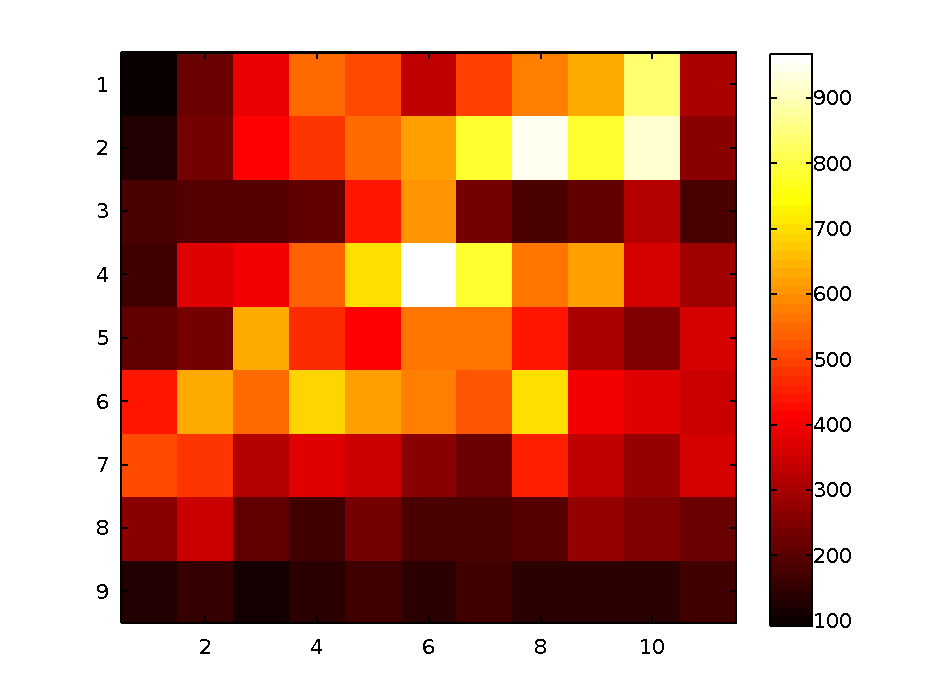
\includegraphics[width=0.47\linewidth]{images/BlockSMCB.pdf}
\label{fig-BlockSMCB}
}
\subfigure[SDMCB des blocs $16\times16$]{
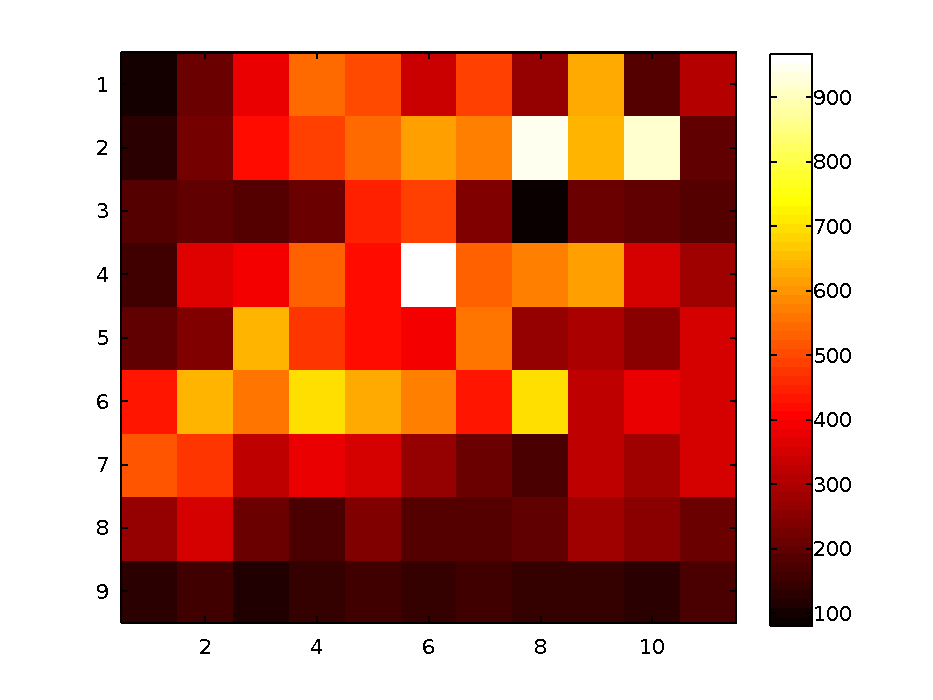
\includegraphics[width=0.47\linewidth]{images/BlockSDMCB.pdf}
\label{fig-BlockSDMCB}
}
\end{varwidth}}
\caption{Approche de détection d'erreur basées sur MCB pour la
\fig{fig-CoastBad}. Pour l'approche SDMCB un seuil $T_b=900$ a été utilisé.}
\label{fig-BlockMCB}
\end{figure}


Nous présentons, à la \fig{fig-BlockMCB}, les résultats obtenus suite à
l'utilisation des approches SMCB et SDMCB sur la trame erronée de la
\fig{fig-CoastBad}. On y constate en \subref{fig-BlockSDMCB} l'élimination de la
propagation des valeurs élevées autour des blocs en erreurs (c.-à-d. SMCB >
800). Lorsque comparé avec l'erreur présente dans la trame
\ref{fig-CoastDiffDiff}, nous sommes en mesure de conclure que l'approche est
supérieure à $\ltD{}$ (voir \fig{fig-BlockDiff}). Pour ce qui est du résiduel,
c'est moins évident. Cependant, l'approche SDMCB~\ref{fig-BlockSDMCB} détecte
non seulement l'erreur prédominante de la trame, mais aussi d'autres
dégradations plus légères qui sont ignorées par le
résiduel~\ref{fig-BlockResidual}. \FloatBarrier
\DIFaddbegin \SC{ pour moi le paragraphe n'est pas très convainquant. c'est difficile de comparer 1.3a, et 1.3b avec 1.6. Devrait-on dire que 3 spots blanc sont identifiés dans 1.6 et que l'un d'entre eux correspond à l'erreur? ou bien que 1.3a identifie un bloc blanc en haut qui n'a pas rapport... Mais c'est difficile de parler de couleurs si le mémoire est imprimé et tons de gris.}


\DIFaddend \end{subsection}

\end{section}

\begin{section}{Les approches sélectives de dissimulation de la détérioration
visuelle.}
\label{sect-Selectives}
Dans cette section, nous sortons du contexte théorique de la détection d'erreurs
et nous offrons une solution pratique de l'application du MCB. Celle-ci a pour
but d'améliorer la qualité visuelle des dissimulations effectuées par le
décodeur de référence H.264. Dans le cadre de nos recherches, nous avons intégré
notre solution au décodeur inclus dans le \ltCodec, mais il est aussi concevable
de le voir comme un module d'extension (\textit{plugiciel}) destiné à d'autres
décodeurs.

L'approche MCB assigne une valeur numérique à un bloc évalué en fonction de
l'écart de son effet de bloc par rapport au bloc qui lui ressemble le plus dans
la trame précédente. Nous affirmons, résultats à l'appui\footnoteETS{Voir le
chapitre Résultats et analyse.}, que cette approche permet d'identifier les
détériorations visuelles importantes dans une trame corrompue. La quantification de
la notion d'une dégradation visuelle importante a été un problème colossal que
nous avons eu à surmonter, lors de notre implémentation pratique.

Une solution simple est l'usage d'un seuil. Cette valeur numérique définit un
point après lequel un bloc avec un certain SDMCB est considéré comme erroné. Ce
type d'approche, employée par \citet{Superiori2007} ainsi que \citet{Ikuno2007},
ne tient pas compte du caractère variant du contenu d'une séquence vidéo.

L'effet de bloc est relatif à l'image dans laquelle il est perçu. Ceci implique
que l'usage d'un seuil fixe ne sera pas en mesure d'identifier les erreurs dans
des séquences où les caractéristiques spatiotemporelles divergent.

De cette observation est née l'approche sélective. Comme son nom l'identique,
cette approche repose sur la notion d'un choix. Ce changement de paradigme
provient du constat suivant : dans un contexte pratique, la dissimulation
est inutile si l'erreur ne peut être dissimulée.
\DIFaddbegin \SC{Phrase bizarre. la détection est inutile?}
\DIFaddend 

En se basant sur le fait que nous cherchons à effectuer une dissimulation, nous
prenons d'un côté une dissimulation traditionnelle, telle la trame calquée ou le
calque des vecteurs de mouvement et nous la comparons à la trame à évaluer. Par
la suite, nous choisissons la plus petite valeur SDMCB. Que ce soit pour une
trame, comme à la section~\ref{sect-SelectiveTrame}, ou pour un macrobloc,
section~\ref{sect-SelectiveBloc}.

Ces approches se comportent comme des seuils dynamiques qui s'adaptent non
seulement au contenu, mais aussi à l'aptitude dissimulation de la détérioration
visuelle. \DIFaddbegin \SC{Phrase bizarre. Revoir à l'aptitude dissimulation de la détérioration} \DIFaddend En effectuant une dissimulation seulement lorsque du contenu de
qualité supérieure (jugée par le SDMCB) est disponible.\DIFaddbegin \SC{Phrase bizarre. Revoir le français de la phrase.} 
\DIFaddend 

Une considération pratique importante est le temps de calcul requis par notre
algorithme. Ce temps est restreint, vu les contraintes temps réel ainsi que les
limitations matérielles des appareils mobiles. Ce qui est dispendieux en terme
de temps de calcul pour le MCB est la recherche des vecteurs de mouvement. Cependant, les
récentes avancées dans ce domaine, telles PMVFAST \citep{Tourapis2001} et
UMHexagonS \citep{Cai2009} réduisent de façon substantielle le temps de calcul
requis pour trouver les vecteurs de mouvement. De plus, notons que dans ce
contexte, le décodeur est informé par les en-têtes RTP des paquets
corrompus et mesure le SDMCB uniquement pour les trames qui en résultent.

\begin{subsection}{L'approche sélective à l'échelon de la trame}
\DIFaddbegin \SC{à l'échel?}\DIFaddend \label{sect-SelectiveTrame}
Notre première approche sélective repose sur le choix d'une trame. Lorsque des
trames sont corrompues, le décodeur peut recourir à plusieurs trames pour la
dissimulation : la tranche calquée, la tranche issue du calque des vecteurs de
mouvement, la trame endommagée. 

Le pointage SDMCB d'une trame est obtenu par la sommation des valeurs du SDMCB
pour chacun de ses macrobloc. Cette sommation est décrite par la formule~:
\begin{equation}
\label{eq-ConcealmentCandidate}
c_c=\sum_{m=0}^{\frac{W}{B}-1}\sum_{n=0}^{\frac{H}{B}-1}\ltSDMCB{\ltConc{}}\:,
\end{equation}
où $\ltConc{}$ est une trame dissimilée par le décodeur, soit par tranche
calquée ou par la tranche issue du calque des vecteurs de mouvement, etc. On
mesure une seconde sommation des valeurs SDMCB pour chaque bloc d'une trame.
Cette fois, nous utilisons la trame endommagée $\ltE{}$~:
\begin{equation}
\label{eq-ErroneousCandidate}
c_e=\sum_{m=0}^{\frac{W}{B}-1}\sum_{n=0}^{\frac{H}{B}-1}\ltSDMCB{\ltE{}}\:,
\end{equation}
Par la suite, la trame avec le plus petit pointage est choisie comme
dissimulation $\ltOpt{}$~:
\begin{equation}
\label{eq-SelectiveConcealment}
\ltOpt{} =
\begin{cases}
\ltE{}, & \mathrm{si~} c_e < c_c\\
\ltConc{}, & \mathrm{sinon}
\end{cases}\:.
\end{equation}

\end{subsection}

\begin{subsection}{L'approche sélective à l'échelon du macrobloc}
\DIFaddbegin \SC{à l'échel?}
\DIFaddend \label{sect-SelectiveBloc}
Notre deuxième approche offre un niveau de granularité supérieur en effectuant
la sélection pour chaque macrobloc. Le but de cette approche est de tirer
profit du gain mutuel de différentes approches en fonction des
caractéristiques spatiotemporelles des régions d'images.

Dans certaines conditions, la tranche calquée est optimale, dans d'autres c'est
la trame erronée ou bien le calque des vecteurs de mouvement. De cette approche
résulte une trame de dissimulation formée d'un conglomérat de macroblocs
optimaux (jugés selon le SDMCB) issus de différentes macroblocs candidats pour la
dissimulation.

La dissimulation résultant de la sélection entre les blocs aux indices $(m,n)$
provenant de la trame corrompue $\ltE{}$ et la trame issue de la dissimulation
par calquage de tranches $\ltConc{}$ est obtenue à l'aide de
\begin{equation}
\label{eq-SelectiveConcealment}
\ltOpt{x,y} =
\begin{cases}
\ltE{x,y}, & \mathrm{si~} \ltSDMCB{\ltE{}} < \ltSDMCB{\ltConc{}}\\
\ltConc{x,y}, & \mathrm{sinon}
\end{cases}\:,
\end{equation}
pour tout $x\in mB+[0,B-1]$, tout $y \in nB+[0,B-1]$, et pour tout bloc de l'image (c.-à-d. $m \in \ltS{m}=[0,\frac{W}{B}-1]$, et $n \in
\ltS{n}=[0,\frac{H}{B}-1]$).
\end{subsection}
\end{section}

Dans ce chapitre, nous avons présenté deux variantes d'un nouveau type
d'algorithme sélectif apte à la dissimulation d'erreurs. Ces variantes agissent
à deux différents échelons de la hiérarchie de la vidéo numérique, soit ceux des
macroblocs et des trames. Pour guider la sélection, nous proposons un algorithme
de détection d'erreurs fondé sur une nouvelle notion: les effets de bloc
compensés par le mouvement. Cette dernière prend en compte une partie des
changements \textit{intertrame}. Ceux-ci, comme nous avons démontré,
entravent à la détection des algorithmes existants.

Le chapitre subséquent porte sur l'analyse des résultats expérimentaux obtenus
à l'aide de notre banc d'essai, conçu pour valider les notions présentées dans
ce chapitre.

\bibliographystyle{bibETS}
\bibliography{mcb}

\end{chapter}

\end{document}